\documentclass[aspectratio=169]{beamer}
\usepackage[utf8]{inputenc}
\usepackage[T1]{fontenc}
\usepackage[brazil]{babel}
\usepackage{ragged2e}
\usepackage{booktabs}
\usepackage{verbatim}
\usepackage{gensymb}
\usepackage{multirow}
\usepackage{xcolor,colortbl}
\definecolor{verde}{rgb}{0,0.5,0}
\usepackage{listings}
\lstset{
  language=C++,
  basicstyle=\ttfamily,
  keywordstyle=\color{blue},
  stringstyle=\color{verde},
  commentstyle=\color{red},
  extendedchars=true,
  showspaces=false,
  showstringspaces=false,
%  numbers=left,
%  numberstyle=\tiny,
  breaklines=true,
  backgroundcolor=\color{green!10},
  breakautoindent=true,
  captionpos=b,
  xleftmargin=0pt
}
\newcommand\setItemnumber[1]{\setcounter{enumi}{\numexpr#1-1\relax}}

\usetheme{AnnArbor}
\usecolortheme{orchid}
\usefonttheme[onlymath]{serif}

\AtBeginSection[]{
  \begin{frame}
  \vfill
  \centering
  \begin{beamercolorbox}[sep=8pt,center,shadow=true,rounded=true]{title}
    \usebeamerfont{title}\insertsectionhead\par%
  \end{beamercolorbox}
  \vfill
  \end{frame}
}

\title[\sc{Makefile e Princípios de POO}]{Makefile e Princípios de Projeto Orientado a Objetos}
\author[Roland Teodorowitsch]{Roland Teodorowitsch}
%\institute[LP2 - EC - PUCRS]{Laboratório de Programação II - Curso de Engenharia de Computação - PUCRS}
\institute[POO - EC - PUCRS]{Programação Orientada a Objetos - ECo - Curso de Engenharia de Computação - PUCRS}
\date{25 de setembro de 2023}

\begin{document}
\justifying

%-------------------------------------------------------
\begin{frame}
	\titlepage
\end{frame}

%=======================================================
\section{Makefile}

%-------------------------------------------------------
\begin{frame}\frametitle{Idéia Geral}
\begin{itemize}
	\item Automatiza a compilação e a geração do executável (``linkar'') de projetos de \emph{software}
	\item Comando:\\\texttt{make}
	\item Arquivo texto contendo as diretivas de compilação e ``linkagem'':\\\texttt{Makefile}
	\item Ao ser chamado, o comando \texttt{make} procura por um arquivo chamado \texttt{Makefile} que diz o que o \texttt{make} deve executar
	\item É padrão no Unix, mas está disponível em outros sistemas
	\item Referência:\\\url{http://mrbook.org/tutorials/make/}
\end{itemize}
\end{frame}

%-------------------------------------------------------
\begin{frame}[fragile]\frametitle{Uso}
\begin{itemize}
	\item Caso \texttt{make} seja executado SEM um alvo (\texttt{make}):
	\begin{itemize}
		\item Se houver \texttt{Makefile}, o rótulo (ou alvo) \texttt{all} será buscado no \texttt{Makefile} para se determinar o que fazer
		\item Se não houver, ocorrerá um erro
	\end{itemize}
	\item Caso \texttt{make} seja executado COM um alvo (\texttt{make \emph{alvo}}):
	\begin{itemize}
		\item Se houver \texttt{Makefile}, o rótulo \texttt{alvo} será buscado no \texttt{Makefile} para se determinar o que fazer
		\item Se não houver, \texttt{make} usará regras internas para criar um executável (\texttt{alvo}) a partir de códigos-fontes (\texttt{alvo.c}, \texttt{alvo.cpp}, etc.) -- ocorrerá um erro se nenhum código-fonte reconhecido for encontrado
	\end{itemize}
	\item Pode-se indicar um arquivo com outro nome (diferente de \texttt{Makefile}) para o \texttt{make}:
\begin{lstlisting}
make -f outro_makefile
\end{lstlisting}
\end{itemize}
\end{frame}

%-------------------------------------------------------
\begin{frame}[fragile]\frametitle{Exemplo de um Projeto de \emph{Software}}
\begin{itemize}
	\item Considere um projeto em C++ formado pelos seguintes arquivos:
	\begin{itemize}
		\item \texttt{main.cpp}: programa principal
		\item \texttt{Data.hpp} e \texttt{Data.cpp}: definição e implementação de uma classe para modelar uma data formada por dia, mês e ano
		\item \texttt{Produto.hpp} e \texttt{Produto.cpp}: definição e implementação da classe para modelar produtos com data de validade
	\end{itemize}
	\item Pode-se gerar um executável chamado \texttt{app} usando:
\begin{lstlisting}
g++ -std=c++11 main.cpp Data.cpp Produto.cpp -o app
\end{lstlisting}
	\item Isto implica compilar sempre tudo a qualquer alteração, o que diminui a escalabilidade
	\item Uma solução mais interessante é criar um \texttt{Makefile} que:
	\begin{itemize}
		\item Compila arquivos \texttt{.cpp} com a opção \texttt{-c} gerando arquivos-objeto (extensão \texttt{.o})
		\item Gera o executável (``linkagem'') a partir dos arquivos-objeto
	\end{itemize}
\end{itemize}
\end{frame}

%-------------------------------------------------------
\begin{frame}[fragile]\frametitle{Formato do \texttt{Makefile}}
\begin{itemize}
	\item Comentários iniciam com \texttt{\#}:
\begin{lstlisting}
# Esta eh uma linha de comentario
# Esta eh outra linha de comentario
\end{lstlisting}
	\item É possível criar variáveis usando \texttt{VARIAVEL=conteudo}, como no \emph{shell script}:
\begin{lstlisting}
# Comando de compilacao
CC=g++
# Flags de compilacao
CFLAGS=-c -std=c++11
\end{lstlisting}
	\item Para acessar o valor da variável basta usar \texttt{\$\{VARIAVEL\}}
\end{itemize}
\end{frame}

%-------------------------------------------------------
\begin{frame}[fragile]\frametitle{Formato do \texttt{Makefile}}
\begin{itemize}
	\item Basicamente o \texttt{Makefile} é formado por regras com o seguinte formato:\\
\texttt{\emph{rótulo}:   \emph{dependências}\\
~ ~ ~ ~ ~\emph{comandos (precedidos de pelo menos um TAB})}
	\item Onde:
	\begin{itemize}
		\item O \emph{rótulo} geralmente é o que se deseja construir e pode ser usado como nome na linha de comando do \texttt{make}
		\item As \emph{dependências} são o que é preciso para se construir o que foi especificado no rótulo
		\item Os \emph{comandos} indicam como construir o rótulo a partir das dependências
	\end{itemize}
	\item Exemplo: gerar um arquivo \texttt{Conta.o} a partir de \texttt{Conta.cpp} e \texttt{Conta.hpp}
\begin{lstlisting}
Produto.o:  Produto.cpp Produto.hpp Data.hpp
            g++ ${CFLAGS} Produto.cpp
\end{lstlisting}
	\item Para ocultar a exibição dos comandos que o \texttt{make} executa, pode-se precedê-los com \texttt{@}
\end{itemize}
\end{frame}

%-------------------------------------------------------
\begin{frame}[fragile]\frametitle{Exemplo Completo}
\begin{lstlisting}[basicstyle=\ttfamily\tiny]
# Makefile (Roland Teodorowitsch; 9 set. 2019)

EXECUTAVEL=app
CFLAGS=-c -std=c++11

all:		${EXECUTAVEL}

${EXECUTAVEL}:	main.o Data.o Produto.o
		@g++ main.o Data.o Produto.o -o ${EXECUTAVEL}

main.o:		main.cpp Data.hpp Produto.hpp
		@g++ ${CFLAGS} main.cpp

Produto.o:	Produto.cpp Produto.hpp Data.hpp
		@g++ ${CFLAGS} Produto.cpp

Data.o:		Data.cpp Data.hpp
		@g++ ${CFLAGS} Data.cpp

run:		${EXECUTAVEL}
		@./${EXECUTAVEL}

clean:
		@rm -f Produto.o Data.o main.o ${EXECUTAVEL}
\end{lstlisting}
\end{frame}

%=======================================================
\section{Princípios de Projeto Orientado a Objetos}

%-------------------------------------------------------
\begin{frame}\frametitle{Princípios de Projeto Orientado a Objetos (POO)}
\begin{itemize}
	\item Os \textbf{objetivos} do projeto de uma classe são construir classes:
	\begin{itemize}
		\item De alta qualidade
		\item Com interfaces públicas consistentes
		\item Úteis e reutilizáveis
	\end{itemize}
	\item Critérios de qualidade da \textbf{interface pública} de uma classe:
	\begin{itemize}
		\item \textbf{Coesão}
		\item Completude
		\item Conveniência
		\item Clareza
		\item Consistência
		\item Acoplamento
		\item \textbf{Encapsulamento}
	\end{itemize}
\end{itemize}
\end{frame}

%=======================================================
\section{Coesão}

%-------------------------------------------------------
\begin{frame}\frametitle{Coesão}
\begin{itemize}
	\item Medida da inter-relação dos membros (atributos e métodos) da interface pública de uma classe
	\item Indica o grau em que uma classe possui uma finalidade única e bem orientada, ou seja, uma classe não deve assumir responsabilidades que não são suas
	\item Na prática:
	\begin{itemize}
		\item Alta coesão é o estado desejável de uma classe cujos membros suportam uma única regra ou responsabilidade bem focada
		\item Baixa coesão é o estado indesejável de uma classe cujos membros suportam múltiplas regras ou responsabilidades desfocadas
	\end{itemize}
\end{itemize}
\end{frame}

%-------------------------------------------------------
\begin{frame}[fragile]\frametitle{Exemplo 1 - Baixa Coesão}
\lstinputlisting[language=C++,basicstyle=\ttfamily\tiny,keywordstyle=\color{red}]{src/Aluno-bc.cpp}
\end{frame}

%-------------------------------------------------------
\begin{frame}[fragile]\frametitle{Exemplo 1 - Alta Coesão}
\begin{columns}
\begin{column}{0.5\linewidth}
\lstinputlisting[language=C++,basicstyle=\ttfamily\tiny,keywordstyle=\color{red}]{src/Aluno-ac.cpp}
\end{column}
\begin{column}{0.5\linewidth}
\lstinputlisting[language=C++,basicstyle=\ttfamily\tiny,keywordstyle=\color{red}]{src/Notas.cpp}
\end{column}
\end{columns}
\end{frame}

%-------------------------------------------------------
\begin{frame}\frametitle{Exemplo 2 - Baixa Coesão}
\begin{columns}
\begin{column}{0.5\linewidth}
\begin{figure}[h]
	\centering
	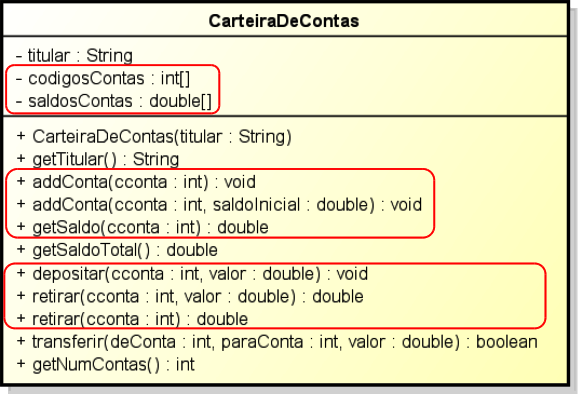
\includegraphics[height=0.45\paperheight]{imagens/carteira.png}
\end{figure}
\end{column}
\begin{column}{0.5\linewidth}
\begin{figure}[h]
	\centering
	
\includegraphics[height=0.075\paperheight]{imagens/classe_nao_coesa.png}
\end{figure}
\begin{itemize}
	\item Esta classe tende a ter dificuldades de manutenção e de reuso!
	\item Devemos ao máximo evitar essas ``super-classes'' que fazem tudo no seu sistema
\end{itemize}
\end{column}
\end{columns}
\end{frame}

%-------------------------------------------------------
\begin{frame}\frametitle{Exemplo 2 - Alta Coesão}
\begin{figure}[h]
	\centering
	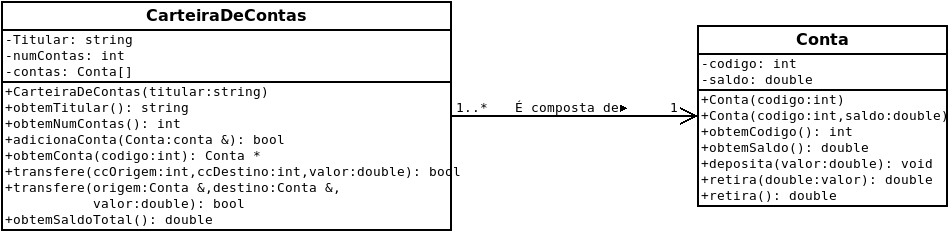
\includegraphics[height=0.3\paperheight]{imagens/carteira_contas.png}
\end{figure}
\begin{itemize}
	\item Classes mais especializadas!
	\item Classes mais fáceis de manter (e menos frequentemente alteradas)
	\item Tendem a ser mais reutilizadas
\end{itemize}
\end{frame}

%=======================================================
\section{Encapsulamento}

%-------------------------------------------------------
\begin{frame}\frametitle{Encapsulamento}
\begin{itemize}
	\item Isolamento do estado interno de uma estrutura de software através de uma interface pública
	\item Encapsular é sinônimo de esconder. Logo, um código encapsulado é aquele código que diz o que faz mas não diz como se faz no primeiro momento. Para saber como faz você deve acessar outro trecho de código. Por isso no encapsulamento devemos prezar pela boa semântica ao darmos nomes aos métodos. Quem lê o nome do método deve saber o que ele faz
	\item Classes bem encapsuladas têm:
	\begin{itemize}
		\item Definição clara da interface pública
		\item Estado interno escondido
	\end{itemize}
	\item A vantagem de uma classe bem encapsulada é que ela simplifica o entendimento do sistema e a manutenção
\end{itemize}
\end{frame}

%-------------------------------------------------------
\begin{frame}\frametitle{Técnica de Anéis de Operações}
\begin{columns}
\begin{column}{0.4\linewidth}
\begin{itemize}
	\item Ajuda a manter um bom encapsulamento interno da classe:
	\begin{itemize}
		\item O uso dessa técnica não afeta o acesso externo (que continua sendo regido por modificadores de visibilidade)
		\item Nessa técnica são criados três anéis fictícios na classe
		\item Os métodos de anéis externos acessam sempre métodos (ou atributos) de anéis internos consecutivos
	\end{itemize}
\end{itemize}
\end{column}
\begin{column}{0.6\linewidth}
\begin{figure}[h]
	\centering
	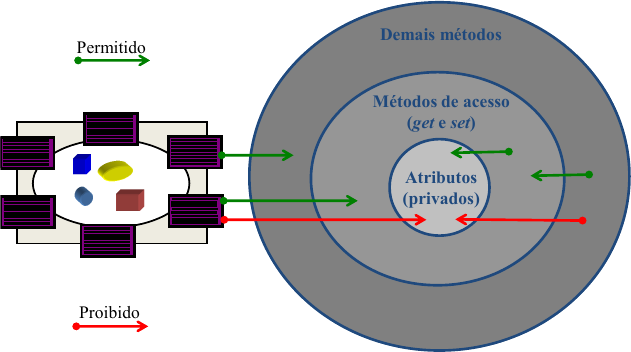
\includegraphics[height=0.5\paperheight]{imagens/aneis.png}
\end{figure}
\end{column}
\end{columns}
\end{frame}

%-------------------------------------------------------
\begin{frame}[fragile]\frametitle{Exemplo}
\begin{columns}
\begin{column}{0.45\linewidth}
\begin{itemize}
	\item Exemplo de bom encapsulamento...
	\begin{figure}[h]
		\centering
		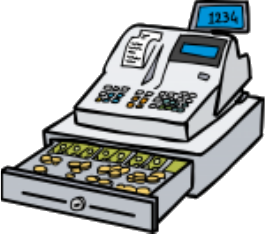
\includegraphics[height=0.2\paperheight]{imagens/caixa.png}
	\end{figure}
	\item Interface Pública bem definida!
	\begin{figure}[h]
		\centering
		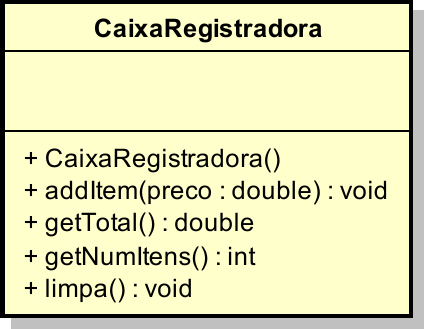
\includegraphics[height=0.3\paperheight]{imagens/caixa_sem_atributos.png}
	\end{figure}
\end{itemize}
\end{column}
\begin{column}{0.55\linewidth}
\begin{itemize}
	\item Exemplo de uso:
\begin{lstlisting}[language=C++,basicstyle=\ttfamily\tiny]
int main() {
  CaixaRegistradora *caixa = new CaixaRegistradora();

  //adiciona tres itens
  caixa->addItem(1.99);
  caixa->addItem(2.99);
  caixa->addItem(1.50);

  cout << caixa->getTotal() << endl;    // saida: 6.48
  cout << caixa->getNumItens() << endl; // saida: 3

  caixa->limpa();

  cout << caixa->getTotal() << endl;    // saida: 0
  cout << caixa->getNumItens() << endl; // saida: 0

  delete caixa;
  return 0;
}
\end{lstlisting}
\end{itemize}
\end{column}
\end{columns}
\end{frame}

%-------------------------------------------------------
\begin{frame}[fragile]\frametitle{Exemplo: Implementação 1}
\begin{columns}
\begin{column}{0.45\linewidth}
\begin{figure}[h]
	\centering
	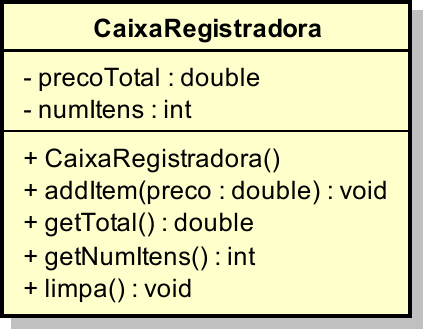
\includegraphics[height=0.3\paperheight]{imagens/caixa_com_atributos.png}
\end{figure}
\end{column}
\begin{column}{0.55\linewidth}
\begin{lstlisting}[language=C++,basicstyle=\ttfamily\tiny]
class CaixaRegistradora {
  private:
    double precoTotal;
    int numItens;
  public:
    CaixaRegistradora() {
      precoTotal = 0.0;
      numItens = 0;
    }
    void addItem(double preco) {
      precoTotal += preco;
      numItens++;
    }
    double getTotal() {
      return precoTotal;
    }
    int getNumItens() {
      return numItens;
    }
    void limpa() {
      precoTotal = 0.0;
      numItens = 0;
    }
};
\end{lstlisting}
\end{column}
\end{columns}
\end{frame}

%-------------------------------------------------------
\begin{frame}[fragile]\frametitle{Implementação 2}
\begin{columns}
\begin{column}{0.45\linewidth}
\begin{itemize}
	\item Quando o encapsulamento é bem feito, pode-se alterar a implementação sem alterar a Interface Pública
	\item O mesmo programa de teste funcionará para as duas implementações
	\begin{figure}[h]
		\centering
		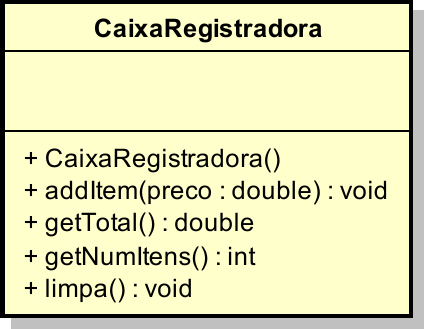
\includegraphics[height=0.3\paperheight]{imagens/caixa_sem_atributos.png}
	\end{figure}
\end{itemize}
\end{column}
\begin{column}{0.55\linewidth}
\begin{lstlisting}[language=C++,basicstyle=\ttfamily\tiny]
class CaixaRegistradora {
private:
   double itens[100];
   int numItens;
public:
   CaixaRegistradora(){
      numItens = 0;
   }
   void addItem(double preco) {
      itens[numItens] = preco;
      numItens++;
   }
   double getTotal() {
      double total = 0;
      for (int i = 0; i < numItens; i++)
          total += itens[i];
      return total;
   }
   int getNumItens() {
      return numItens;
   }
   void limpa() {
      numItens = 0;
   }
};
\end{lstlisting}
\end{column}
\end{columns}
\end{frame}

%-------------------------------------------------------
\begin{frame}[fragile]\frametitle{Comparando as 2 Implementações...}
\begin{columns}
\begin{column}{0.5\linewidth}
\begin{lstlisting}[language=C++,basicstyle=\ttfamily\tiny]
class CaixaRegistradora {
private:
   double precoTotal;
   int numItens;
public:
   CaixaRegistradora() {
      precoTotal = 0.0;
      numItens = 0;
   }
   void addItem(double preco) {
      precoTotal += preco;
      numItens++;
   }
   double getTotal() {
      return precoTotal;
   }
   int getNumItens() {
      return numItens;
   }
   void limpa() {
      precoTotal = 0.0;
      numItens = 0;
   }
};
\end{lstlisting}
\end{column}
\begin{column}{0.5\linewidth}
\begin{lstlisting}[language=C++,basicstyle=\ttfamily\tiny]
class CaixaRegistradora {
private:
   double itens[100];
   int numItens;
public:
   CaixaRegistradora(){
      numItens = 0;
   }
   void addItem(double preco) {
      itens[numItens] = preco;
      numItens++;
   }
   double getTotal() {
      double total = 0;
      for (int i = 0; i < numItens; i++)
          total += itens[i];
      return total;
   }
   int getNumItens() {
      return numItens;
   }
   void limpa() {
      numItens = 0;
   }
};
\end{lstlisting}
\end{column}
\end{columns}
\end{frame}

%=======================================================
\section{Lista de Exercícios}

%-------------------------------------------------------
\begin{frame}\frametitle{Exercício 1}
\begin{enumerate}
	\setItemnumber{1}
	\item Uma livraria possui alguns produtos à venda, como livros, cadernos, calendários e canetas. Todos os produtos possuem nome e preço. Cadernos possuem também o número de páginas, como os livros e calendários, mas estes últimos se diferenciam por ainda terem o atributo ano. Esta loja é conhecida pelas promoções que oferece. Uma promoção Regular oferece um desconto de 10\% em cada produto. Já a Liquidação oferece um desconto de 30\% no preço de cada produto.
\begin{columns}
\begin{column}{0.4\linewidth}
\begin{figure}[h]
	\centering
	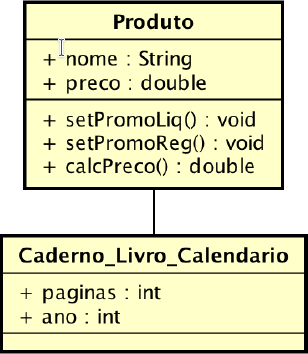
\includegraphics[height=0.35\paperheight]{imagens/modelagem_livraria.png}
\end{figure}
\end{column}
\begin{column}{0.6\linewidth}
\begin{itemize}
	\item Um colega apresentou a modelagem UML ao lado, e pediu para você verifica-la. Logo, você deve melhorar a modelagem do seu colega sempre pensando em termos classes encapsuladas com alta coesão! Além de implementa-las, é claro!
\end{itemize}
\end{column}
\end{columns}
\end{enumerate}
\end{frame}

%-------------------------------------------------------
\begin{frame}\frametitle{Exercício 1 - Exemplo de Modelagem}
\begin{figure}[h]
	\centering
	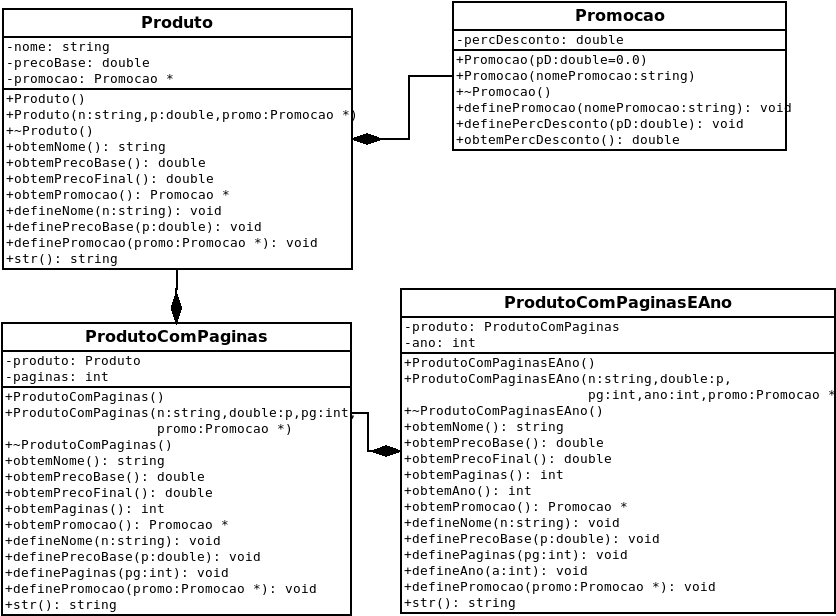
\includegraphics[height=0.7\paperheight]{imagens/modelagem_livraria2.png}
\end{figure}
\end{frame}

%-------------------------------------------------------
\begin{frame}\frametitle{Exercício 2}
\begin{enumerate}
	\setItemnumber{2}
	\item Crie um programa que gerencie uma turma de determinada disciplina, contendo professor, alunos e recursos utilizados. O relacionamento entre as classes que deverão ser implementadas é mostrado no diagrama de classes da próxima página.
	\begin{itemize}
		\item Uma turma pode ter no máximo 30 alunos matriculados.
		\item Uma turma pode ter no máximo 5 recursos alocados.
		\item Para testar a implementação, no programa principal (função \texttt{main()}), crie uma instância da classe \texttt{Turma}, e preencha-a com referências para objetos das classes \texttt{Professor}, \texttt{Aluno} (4 alunos) e \texttt{Recurso} (3 recursos). Inicialize estes objetoss na função \texttt{main()} e implemente os métodos \texttt{str()} das classes para que sejam mostradas as informações dos objetos como ilustrado no exemplo de execução que aparece logo após o diagrama de classes.
	\end{itemize}
\end{enumerate}
\end{frame}

%-------------------------------------------------------
\begin{frame}\frametitle{Exercício 2: Diagrama de Classes}
\begin{figure}[h]
	\centering
	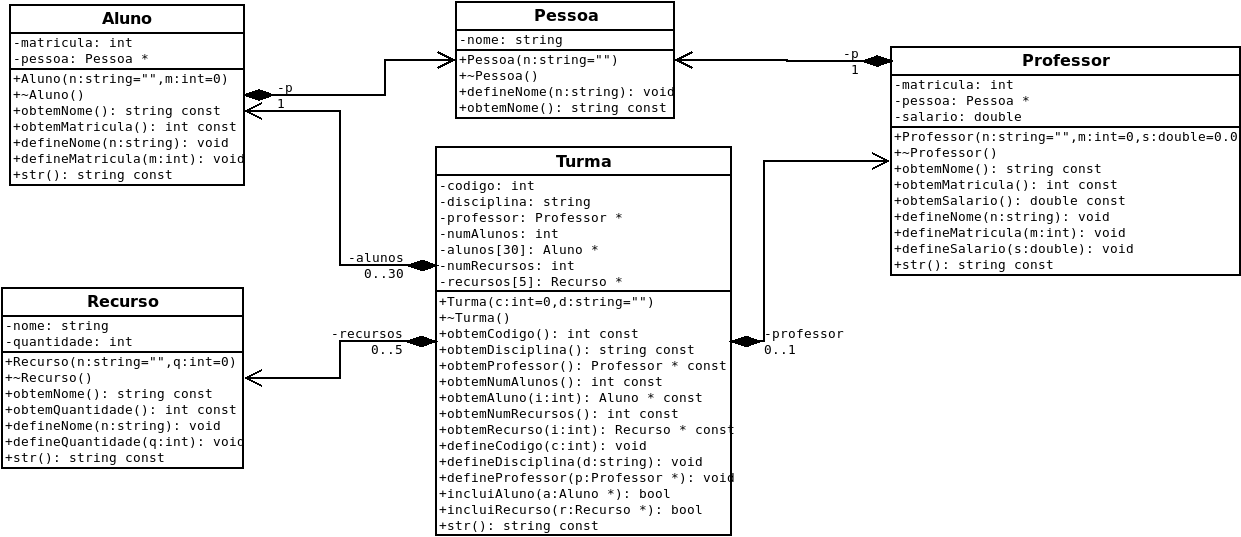
\includegraphics[height=0.7\paperheight]{imagens/modelagem_turma.png}
\end{figure}
\end{frame}

%-------------------------------------------------------
\begin{frame}[fragile]\frametitle{Exercício 2: Exemplo de Execução}
\lstinputlisting{src/exercicio2/app.out}
\end{frame}

%=======================================================
\section{Créditos}

%-------------------------------------------------------
\begin{frame}\frametitle{Créditos}
\begin{itemize}
	\item Estas lâminas contêm trechos de materiais disponibilizados pelo professor Rafael Garibotti.
\end{itemize}
\end{frame}

%=======================================================
\section{Soluções}

%-------------------------------------------------------
\begin{frame}[fragile]\frametitle{Exercício 2: \texttt{Pessoa.hpp}}
\lstinputlisting[basicstyle=\ttfamily\tiny]{src/exercicio2/Pessoa.hpp}
\end{frame}

%-------------------------------------------------------
\begin{frame}[fragile]\frametitle{Exercício 2: \texttt{Pessoa.cpp}}
\lstinputlisting[basicstyle=\ttfamily\tiny]{src/exercicio2/Pessoa.cpp}
\end{frame}

%-------------------------------------------------------
\begin{frame}[fragile]\frametitle{Exercício 2: \texttt{Aluno.hpp}}
\lstinputlisting[basicstyle=\ttfamily\tiny]{src/exercicio2/Aluno.hpp}
\end{frame}

%-------------------------------------------------------
\begin{frame}[fragile]\frametitle{Exercício 2: \texttt{Aluno.cpp}}
\fontsize{6pt}{6pt}\selectfont{
\lstinputlisting{src/exercicio2/Aluno.cpp}
}
\end{frame}

%-------------------------------------------------------
\begin{frame}[fragile]\frametitle{Exercício 2: \texttt{Professor.hpp}}
\lstinputlisting[basicstyle=\ttfamily\tiny]{src/exercicio2/Professor.hpp}
\end{frame}

%-------------------------------------------------------
\begin{frame}[fragile]\frametitle{Exercício 2: \texttt{Professor.cpp}}
\fontsize{5pt}{5pt}\selectfont{
\lstinputlisting{src/exercicio2/Professor.cpp}
}
\end{frame}

%-------------------------------------------------------
\begin{frame}[fragile]\frametitle{Exercício 2: \texttt{Recurso.hpp}}
\lstinputlisting[basicstyle=\ttfamily\tiny]{src/exercicio2/Recurso.hpp}
\end{frame}

%-------------------------------------------------------
\begin{frame}[fragile]\frametitle{Exercício 2: \texttt{Recurso.cpp}}
\fontsize{6pt}{6pt}\selectfont{
\lstinputlisting{src/exercicio2/Recurso.cpp}
}
\end{frame}

%-------------------------------------------------------
\begin{frame}[fragile]\frametitle{Exercício 2: \texttt{Turma.hpp}}
\fontsize{5pt}{5pt}\selectfont{
\lstinputlisting{src/exercicio2/Turma.hpp}
}
\end{frame}

%-------------------------------------------------------
\begin{frame}[fragile]\frametitle{Exercício 2: \texttt{Turma.cpp} (primeira parte)}
\fontsize{6pt}{6pt}\selectfont{
\lstinputlisting[firstline=1,lastline=32]{src/exercicio2/Turma.cpp}
}
\end{frame}

%-------------------------------------------------------
\begin{frame}[fragile]\frametitle{Exercício 2: \texttt{Turma.cpp} (segunda parte)}
\fontsize{6pt}{6pt}\selectfont{
\lstinputlisting[firstline=33]{src/exercicio2/Turma.cpp}
}
\end{frame}

%-------------------------------------------------------
\begin{frame}[fragile]\frametitle{Exercício 2: \texttt{main.cpp}}
\fontsize{6pt}{6pt}\selectfont{
\lstinputlisting{src/exercicio2/main.cpp}
}
\end{frame}

%-------------------------------------------------------
\begin{frame}[fragile]\frametitle{Exercício 2: \texttt{Makefile}}
\lstinputlisting[basicstyle=\ttfamily\tiny]{src/exercicio2/Makefile}
\end{frame}


%-------------------------------------------------------
\end{document}

